
\section{Suffix Trie/Array} % (6.6)

\begin{frame}
  \begin{center}
    {\bf Part III: Suffix Tree, Array}
  \end{center}
\end{frame}


\subsection{Outline}
\begin{frame}
  \frametitle{Suffix Trie: Definition}

  {\smaller
    \begin{block}{}
      Data structure used to find matching suffixes of multiple strings.
    \end{block}

    \vfill

    \begin{center}
    \structure{Suffix Trie for \{'CAR','CAT','RAT'\}}
    \end{center}

    \vfill

    \begin{columns}[T]
      \column{0.25\textwidth}
      All Suffixes
      \begin{enumerate}
      \item CAR
      \item AR
      \item R
      \item CAT
      \item T
      \item RAT
      \item AT
      \item T
      \end{enumerate}
      \column{0.25\textwidth}
      Sorted, Unique Suffixes
      \begin{enumerate}
      \item AR
      \item AT
      \item CAR
      \item CAT
      \item R
      \item RAT
      \item T (x2)
      \end{enumerate}
      \column{0.45\textwidth}
      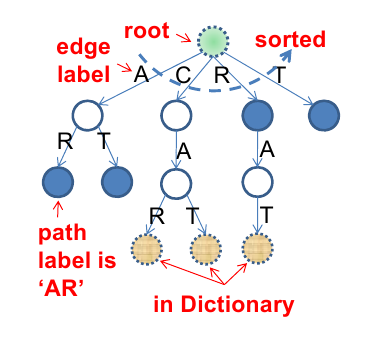
\includegraphics[width=.9\textwidth]{../img/suffixtrie_halim}\\
      % TODO: Replace suffix trie image with one of my own design
    \end{columns}
  }
\end{frame}

\begin{frame}
  \frametitle{Suffix Trie: Counting the number of substrings of GATAGACA}
  \begin{columns}[T]
    \column{0.5\textwidth}
    {\smaller
    Create all $n$ suffixes:

    \begin{tabular}{c|l}
      i & suffix\\
      \hline
      0 & GATAGACA\$\\
      1 & ATAGACA\$\\
      2 & TAGACA\$\\
      3 & AGACA\$\\
      4 & GACA\$\\
      5 & ACA\$\\
      6 & CA\$\\
      7 & A\$\\
      8 & \$\\
    \end{tabular}\bigskip

    Number of repeats of substring $m$:
    \begin{itemize}
    \item 'A': 4 subtrees
    \item 'GA': 2 subtrees
    \item 'AA': 0 subtrees
    \end{itemize}}
    \column{0.5\textwidth}
    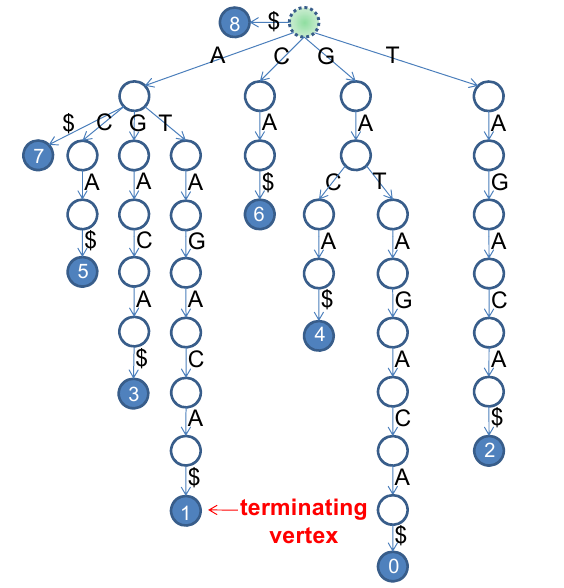
\includegraphics[width=.85\textwidth]{../img/suffixtrie_halim2}
  \end{columns}
\end{frame}

\begin{frame}
  \frametitle{Suffix Trie: Counting the number of substrings of GATACA}
  \begin{columns}[T]
    \column{0.5\textwidth}

    {\smaller

    You can make the Suffix Tree better by merging the nodes that have a single child.\bigskip

    This data structure is useful for many algorithms.\bigskip

    \begin{tabular}{c|l}
      i & suffix\\
      \hline
      0 & GATAGACA\$\\
      1 & ATAGACA\$\\
      2 & TAGACA\$\\
      3 & AGACA\$\\
      4 & GACA\$\\
      5 & ACA\$\\
      6 & CA\$\\
      7 & A\$\\
      8 & \$\\
    \end{tabular}
    }

    \column{0.5\textwidth}
    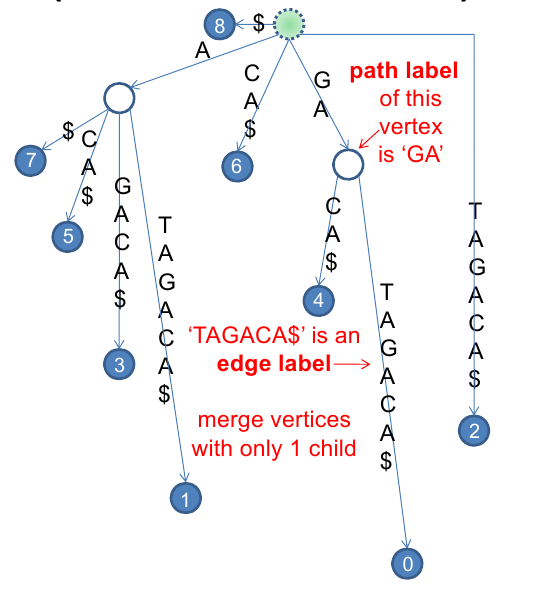
\includegraphics[width=.8\textwidth]{../img/suffixtree_halim}
    \ppagenote{Suffix Tree/Array images from Steven Halim, "Competitive Programming 3", chapter 6.6}
  \end{columns}
\end{frame}

\subsection{Uses of a Suffix Tree}
\begin{frame}
  \frametitle{Uses of a Suffix Tree 1: String Matching} {\smaller

    \structure{Assuming that we have the Suffix Tree already built},
    we can find all occurrences of substring $m$ in $T$ in time
    $O(m+\text{occ})$, where occ is the number of occurrences.

  \begin{center}
    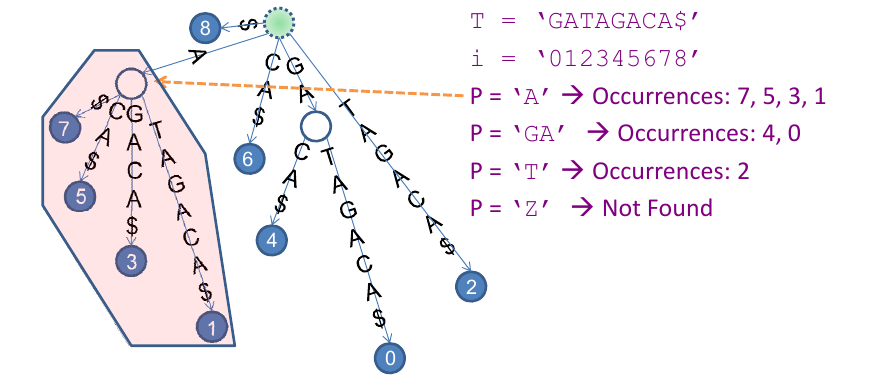
\includegraphics[width=0.9\textwidth]{../img/stringmatching_halim}
  \end{center}
  }
\end{frame}

\begin{frame}
  \frametitle{Uses of a Suffix Tree 2: Longest Repeated Substring}
  \begin{itemize}
  \item The LRS is the longest substring with number of occurrences $> 2$;
  \item The LRS is the deepest {\bf internal node} in the tree;
  \end{itemize}

  \begin{center}
    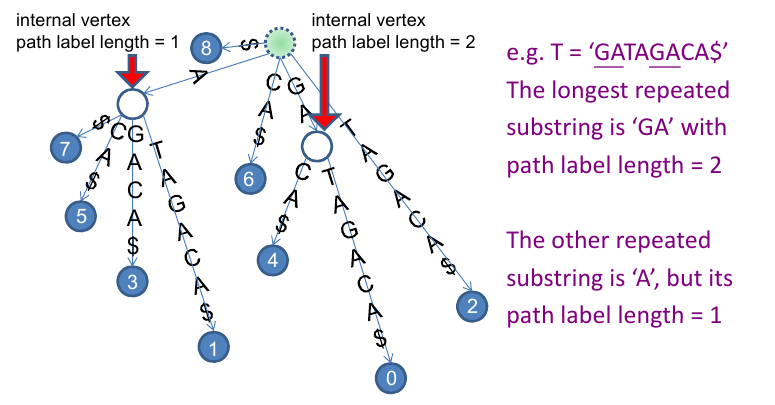
\includegraphics[width=0.75\textwidth]{../img/longestrepeatingsubstring_halim}
  \end{center}
\end{frame}

\begin{frame}
  \frametitle{Uses of a Suffix Tree 3: Longest Common Substring}
    \begin{itemize}
    \item Make a Suffix Tree of $M$ and $N$ combined, with a different ending character to each.
    \item The LCS is the deepest {\bf internal node} that includes both ending characters.
    \end{itemize}
  \begin{center}
    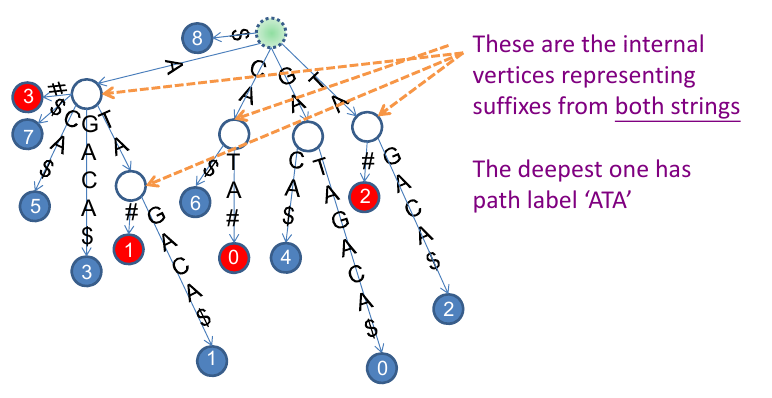
\includegraphics[width=0.75\textwidth]{../img/longestcommonsubstring_halim}
  \end{center}
\end{frame}

\subsection{Suffix Array}
\begin{frame}
  \frametitle{Suffix Array}
  \begin{itemize}
    \item The algorithms in previous slides are very efficient...\\
      ... \structure{if you have the suffix tree}

      \medskip

    \item The suffix tree can be built in $O(n)$...\\
      ... but implementation is rather complex;

      \medskip

    \item In this course, we will see the \structure{Suffix Array};

      \medskip

    \item The Suffix Array is built in $O(n\log{n})$...\\
      ... but the implementation is very simple!
  \end{itemize}

  \vfill

  \begin{block}{}
    I encourage you to study the implementation of the suffix tree by yourself!
  \end{block}
\end{frame}

\begin{frame}
  \frametitle{Suffix Array Implementation Idea}

    \begin{itemize}
    \item To make a Suffix array, make an array of all possible
      suffixes of $T$, and sort it;
    \item The order of the suffix array is the
      \structure{visit in preorder} of the suffix tree;
      % TODO: Japanese for pre-order visit
    \item We can adapt all algorithms accordingly;
    \end{itemize}

  \begin{columns}
    \column{0.4\textwidth}
    \begin{tabular}{c|l}
      i & suffix\\
      \hline
      0 & GATAGACA\$\\
      1 & ATAGACA\$\\
      2 & TAGACA\$\\
      3 & AGACA\$\\
      4 & GACA\$\\
      5 & ACA\$\\
      6 & CA\$\\
      7 & A\$\\
      8 & \$\\
    \end{tabular}
    \column{0.2\textwidth}
    Sort $\rightarrow$
    \column{0.4\textwidth}
    \begin{tabular}{c|c|l}
      i & SA[i] & suffix \\
      \hline
      0 & 8 & \$\\
      1 & 7 & A\$\\
      2 & 5 & ACA\$\\
      3 & 3 & AGACA\$\\
      4 & 1 & ATAGACA\$\\
      5 & 6 & CA\$\\
      6 & 4 & GACA\$\\
      7 & 0 & GATAGACA\$\\
      8 & 2 & TAGACA\$\\
    \end{tabular}
  \end{columns}
\end{frame}

\begin{frame}[fragile]
  \frametitle{Suffix Array: Slow Implementation}
  {\smaller
    \begin{exampleblock}{Simple Implementation}
\begin{verbatim}
#include <algorithm>
#include <cstdio>
#include <cstring>
using namespace std;
char T[MAX_N]; int SA[MAX_N],i,n;

bool cmp(int a, int b) { return strcmp(T+a, T+b) < 0; }
// O(n)

int main() {
  n = (int) strlen (gets(T));
  for (int i = 0; i < n; i++) SA[i] = i;
  sort (SA, SA+n, cmp); // O(n^2 log n) }
\end{verbatim}
\end{exampleblock}}

    This implementation is too slow for strings bigger than 1000 characters.
\end{frame}

\begin{frame}[fragile]
  \frametitle{Suffix Array: Better Implementation (1)}
  {\smaller
    \begin{exampleblock}{O(n log n) implementation using ``ranking pairs/radix sort''}
\begin{verbatim}
char T[MAX_N]; int n; int c[MAX_N];
int RA[MAX_N], tempRA[MAX_N], SA[MAX_N], tempSA[MAX_N];

void countingSort(int k) {
  int i, sum, maxi = max(300,n);                        //255 ASCII chars or n
  memset(c, 0, sizeof(c));
  for (i = 0; i < n; i++) c[i+k<n? RA[i+k] : 0]++
  for (i = sum = 0; i < maxi; i++)
    { int t = c[i]; c[i] = sum; sum += t; }             //frequency
  for (i = 0; i < n; i++)
    tempSA[c[SA[i]+k < n ? RA[SA[i]+k] : 0]++] = SA[i];
  for (i = 0; i < n; i++)                               // update suffix array
    SA[i] = tempSA[i];
}

// ... continues next slide
\end{verbatim}
    \end{exampleblock}
  }
\end{frame}

\begin{frame}[fragile]
  \frametitle{Suffix Array: Better Implementation (2)}
  {\smaller
    \begin{exampleblock}{O(n log n) implementation using ``ranking pairs/radix sort''}
\begin{verbatim}
// ... continued from last slide
void constructSuffixArray() {
  int i, k, r;
  for (i = 0; i < n; i++) { RA[i] = T[i]; SA[i] = i;}
  for (k = 1; k < n; k <<=1) {
    countingSort(k); countingSort(0); tempRA[SA[0]] = r = 0;
    for (i = 1; i < n; i++)
      tempRA[SA[i]] =
          (RA[SA[i]] == RA[SA[i-1]] && RA[SA[i]+k] == RA[SA[i-1]+k]) ?
           r : ++r;
    for (i = 0; i < n; i++)
      RA[i] = tempRA[i];
    if (RA[SA[n-1]] == n-1) break;
  }
}
\end{verbatim}
    \end{exampleblock}
  }
\end{frame}

\begin{frame}
  \frametitle{Using Suffix Array for String Matching:}
  {\smaller
    \begin{block}{}
      \begin{itemize}
      \item Do binary search two times: One to find the lower bound, one to find the upper bound;
      \end{itemize}
    \end{block}
    \begin{center}
      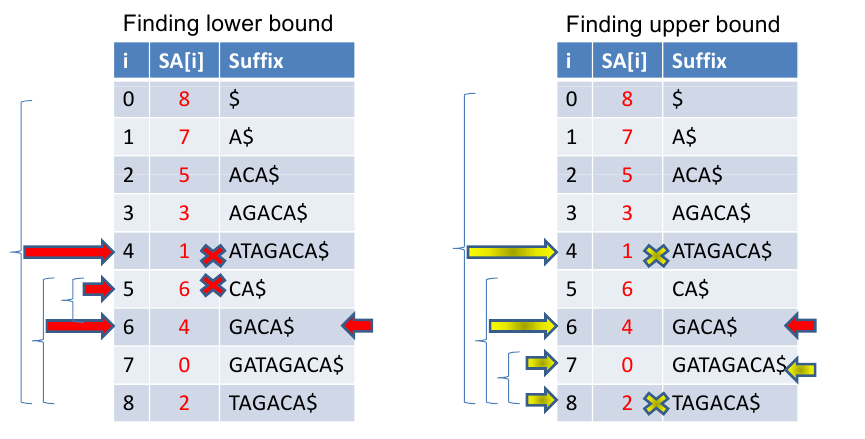
\includegraphics[width=0.8\textwidth]{../img/suffixarray_halim}
    \end{center}
  }
\end{frame}

\begin{frame}{Using Suffix Array for Longest Repeated Substring}
  {Find the pair of indexes $i$ and $i+i$ with longest common prefix.}

    \begin{center}
      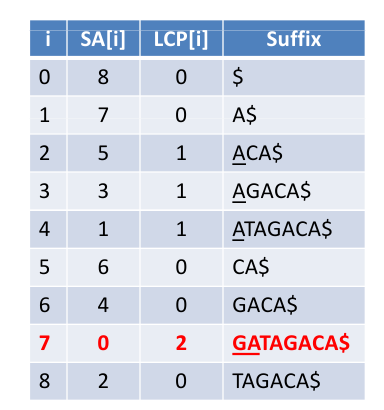
\includegraphics[width=0.4\textwidth]{../img/suffixarray2_halim}
    \end{center}
\end{frame}

\begin{frame}{Using Suffix Array for Longest Common Substring}
  {Append strings $M$ and $N$ with different endings, and find LCS}
    \begin{center}
      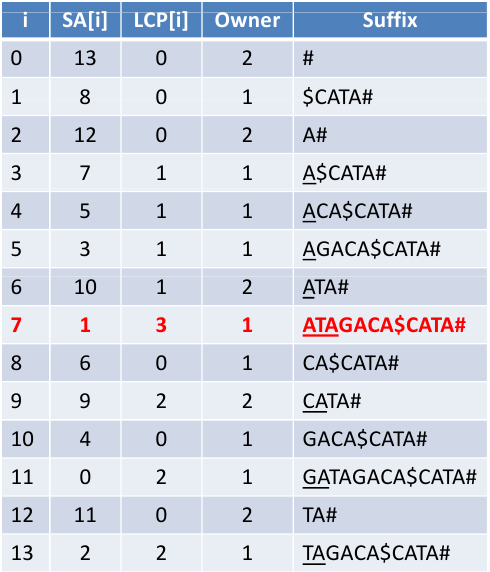
\includegraphics[width=0.36\textwidth]{../img/suffixarray3_halim}
    \end{center}
\end{frame}
